\chapter{lilypond}
\section*{Écriture de partitions}
Les partitions pour la description des systèmes et les transcriptions manuelles sont écrites avec LilyPond.\\\\
Le fichier description\_notation.ly :
\begin{verbatim}
\version "2.22.1"
\language français
\include "../0_drum_style_perso.ly"

up = {
\clef percussion
\override Staff.TimeSignature.stencil = ##f
\x do''4-"rd" s s s \c la'4-"co" s s s \x la'4-"cf" s s s \o fa'4-"ta" s s s do'-"cc" s s s \x do'-"xo" s s s
}
down = {
\clef percussion
\override Staff.TimeSignature.stencil = ##f
s s s s s
}
\score 
{
<<
\new Staff
<<
\new Voice { \voiceOne \up }
\new Voice { \voiceTwo \down }
>>
\addlyrics { "Voix haute." }
>>
}

up = {
\clef percussion
\override Staff.TimeSignature.stencil = ##f
s s s s s
}
down = {
\clef percussion
\override Staff.TimeSignature.stencil = ##f
\x do4-"pf" s s s \c do4-"po" s s s \o mi-"gc" s s s sol-"tb" s s s do'-"cc" s s s \x do'-"xo" s s s
}
\score 
{
<<
\new Staff
<<
\new Voice { \voiceOne \up }
\new Voice { \voiceTwo \down }
>>
\addlyrics { "Voix basse." }
>>
}
\end{verbatim}
Et le fichier 0\_drum\_style\_perso.ly :
\begin{verbatim}
\version "2.22.1"
\language français

% LES TÊTES DE NOTES

% Standards noteheads
o = {
\revert NoteHead.style
}

% Cymbales, HH, or cross-stick
x = {
\override NoteHead.style = #'cross
}

% Open HH
c = {
\override NoteHead.style = #'xcircle
}

% Ghost notes
g = {
\override NoteHead.style = #'harmonic
}

% Caisse claire : \o + do'
% Cross stick : \x + do'
% Grosse caisse : \o + mi
% Ride : \x + do''
% Charley : \x + la'
% Charley ouvert : \c + la'
% Charley au pied : \x + do
% Charley ouvert au pied : \c + do

% FLAS

% Flas caisse-claire
fla_cc = {
\appoggiatura do'8 do'4
}
\end{verbatim}
Ces scripts génèrent le document suivant :\\
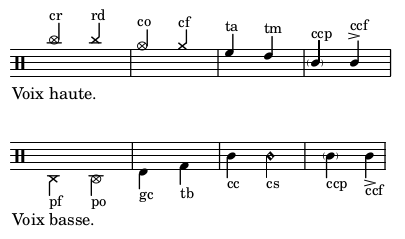
\includegraphics[height=50mm, width=110mm]{images/notation/description_notation.png}\\\\
\textbf{Bases :}\\
\url{http://lilypond.org/doc/v2.22/Documentation/learning/simple-notation}\\

\textbf{Percussions et batterie :}\\
\url{http://lilypond.org/doc/v2.22/Documentation/notation/common-notation-for-percussion}\\

